
\documentclass{article}

\usepackage[utf8]{inputenc}

\usepackage{amsmath, bm}
\usepackage{graphicx}
\usepackage{amssymb}
\usepackage{float}
\usepackage{caption}
\usepackage{subcaption}
\usepackage{hyperref}
\usepackage{tikz}
\usepackage{layout}

\usepackage[margin=1in]{geometry}
\usepackage{listings}
\usepackage{xcolor}
\usepackage{color, colortbl}
\usepackage{textgreek}
\usepackage{mathrsfs}
\usepackage{savetrees}

\usepackage{titlesec}

\titleformat{\subsubsection}
  {\normalfont\selectfont}{\thesubsubsection}{1em}{}

\usetikzlibrary{calc}
\usetikzlibrary{angles,quotes} % for pic
\usetikzlibrary{patterns,snakes}
\usetikzlibrary{arrows}
\tikzset{>=latex} % for LaTeX arrow head

\setlength{\parskip}{\baselineskip}%
\setlength{\parindent}{0pt}%
\linespread{0.9}


\definecolor{codegreen}{rgb}{0,0.6,0}
\definecolor{codegray}{rgb}{0.5,0.5,0.5}
\definecolor{codepurple}{rgb}{0.58,0,0.82}
\definecolor{backcolour}{rgb}{0.95,0.95,0.92}

\lstdefinestyle{mystyle}{
    backgroundcolor=\color{backcolour},   
    commentstyle=\color{codegreen},
    keywordstyle=\color{magenta},
    numberstyle=\tiny\color{codegray},
    stringstyle=\color{codepurple},
    basicstyle=\ttfamily\footnotesize,
    breakatwhitespace=false,         
    breaklines=true,                 
    captionpos=b,                    
    keepspaces=true,                 
    numbers=left,                    
    numbersep=5pt,                  
    showspaces=false,                
    showstringspaces=false,
    showtabs=false,                  
    tabsize=2
}

\lstset{style=mystyle}


\begin{document}

\title{4C8: Model Tyre Tests}
\author{lwp26}
\date{November 2024}
\maketitle 

\iffalse
\begin{abstract}
    \centering
    LOg bAs
\end{abstract}
\fi

%-----------------------------------------------------------------------------------------
\section{Introduction}
%-----------------------------------------------------------------------------------------

\subsection{Objectives}

\begin{itemize}
    \item A static tyre and rolling road test rig will be calibrated and tested to verify invariance of forces with speed to allow manual movements of the road surface.
    \item The normal load on the tyre will be varied to understand its impact on the steady state lateral force.
    \item The longitudinal creepage of the tyre will be measured by applying a torque at 0 steer angle.
    \item The combined lateral and longitudinal creepage of the tyre will be measured by applying varying torques at two steer angles.
    \item These combined results will be compared to theoretical models obtained by the individual creep experiments.
\end{itemize}

\subsection{Setup}

\begin{figure}[H]
    \centering
    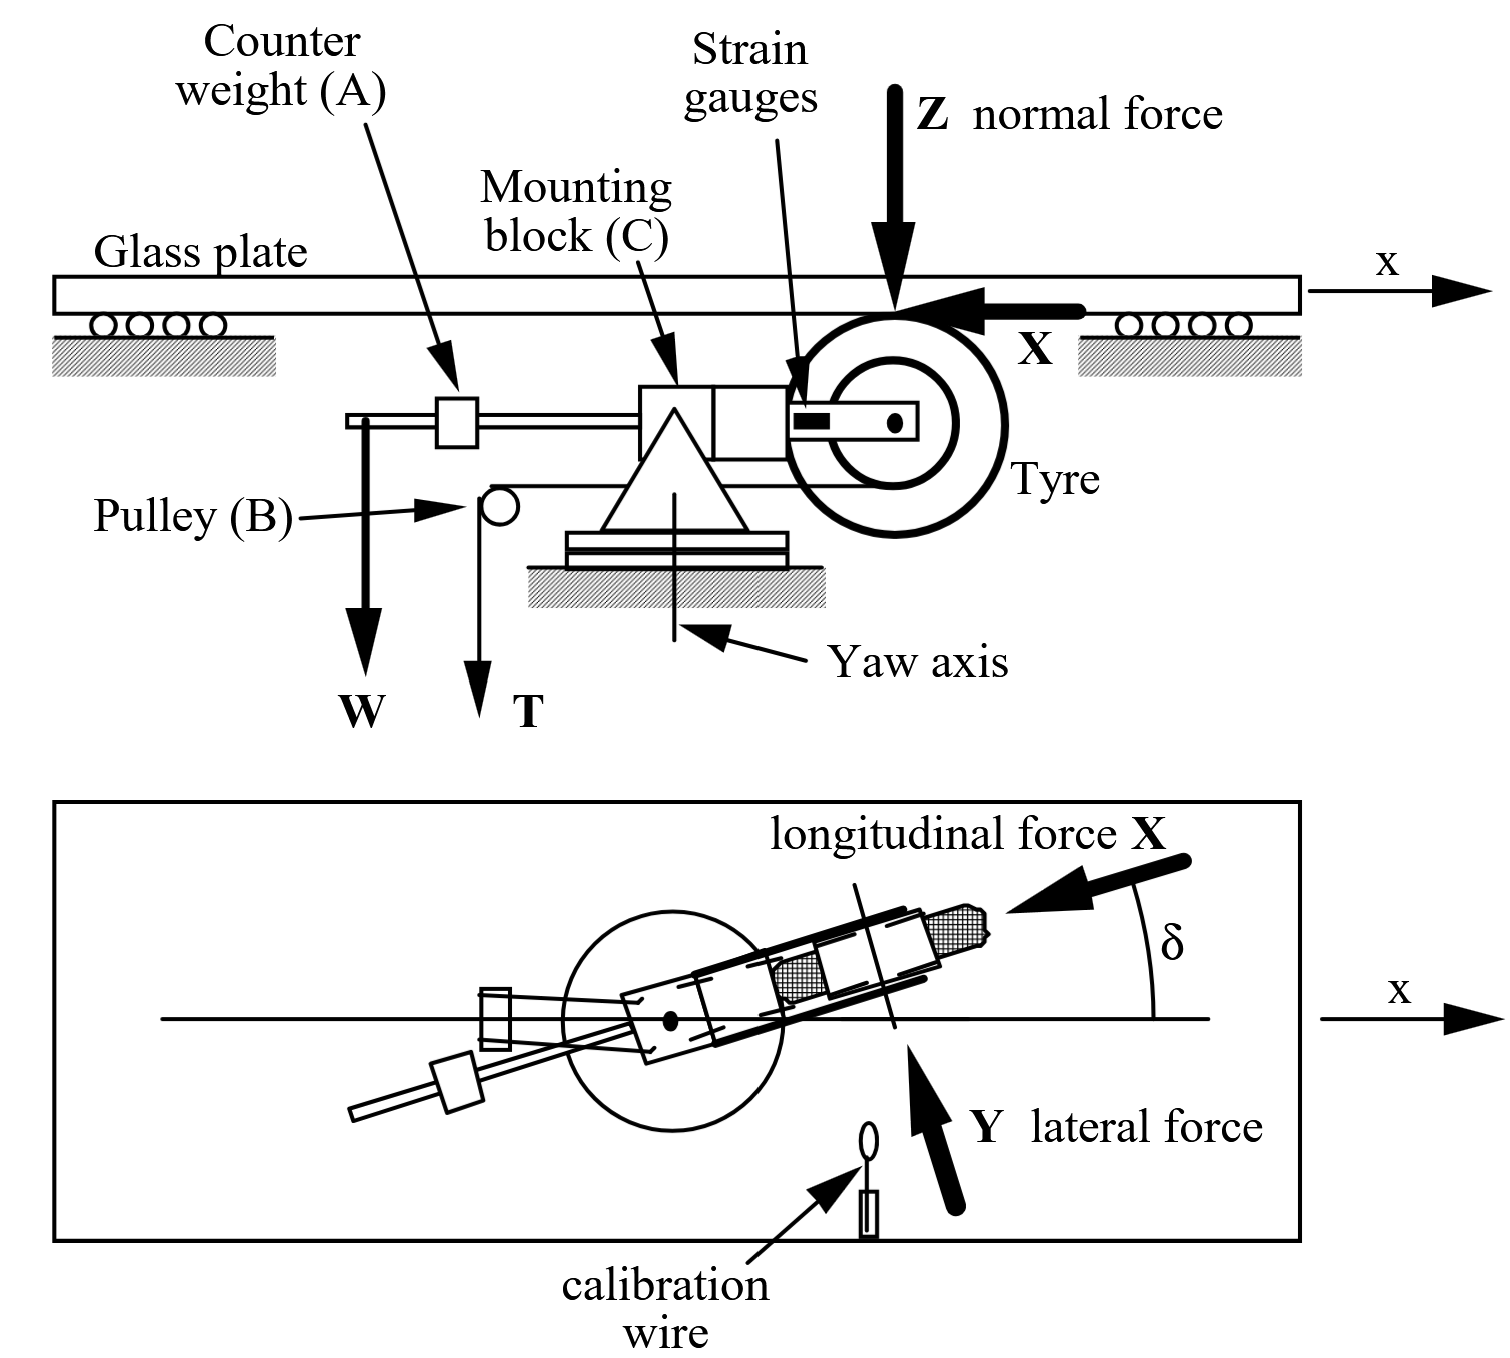
\includegraphics[width=0.7\textwidth]{photos/setup.png}
    \caption{The experimental setup.}
    \label{fig:setup}
\end{figure}

The normal force Z is applied by a mass on a lever arm and is calculated using the equation below.
\begin{equation}
    Z = W * \frac{r_{\text{lever}}}{r_{\text{wheel}}}
\end{equation}
The longitudinal force X is applied by wire wound around a drum and is calculated using the equation below.
\begin{equation}
    X = T * \frac{r_{\text{drum}}}{r_{\text{wheel}}}
\end{equation}
The effective radius of the wheel varies on the normal force, as the wheel deforms more under higher loads.
This radius was measured by measuring the distance the unyawed wheel travelled with no load applied which can be seen in section \ref{no_load_creep}.

\section{LATERAL CREEP}

\subsection{\textbf{Transducer Calibration}}

\begin{figure}[H]
    \centering
    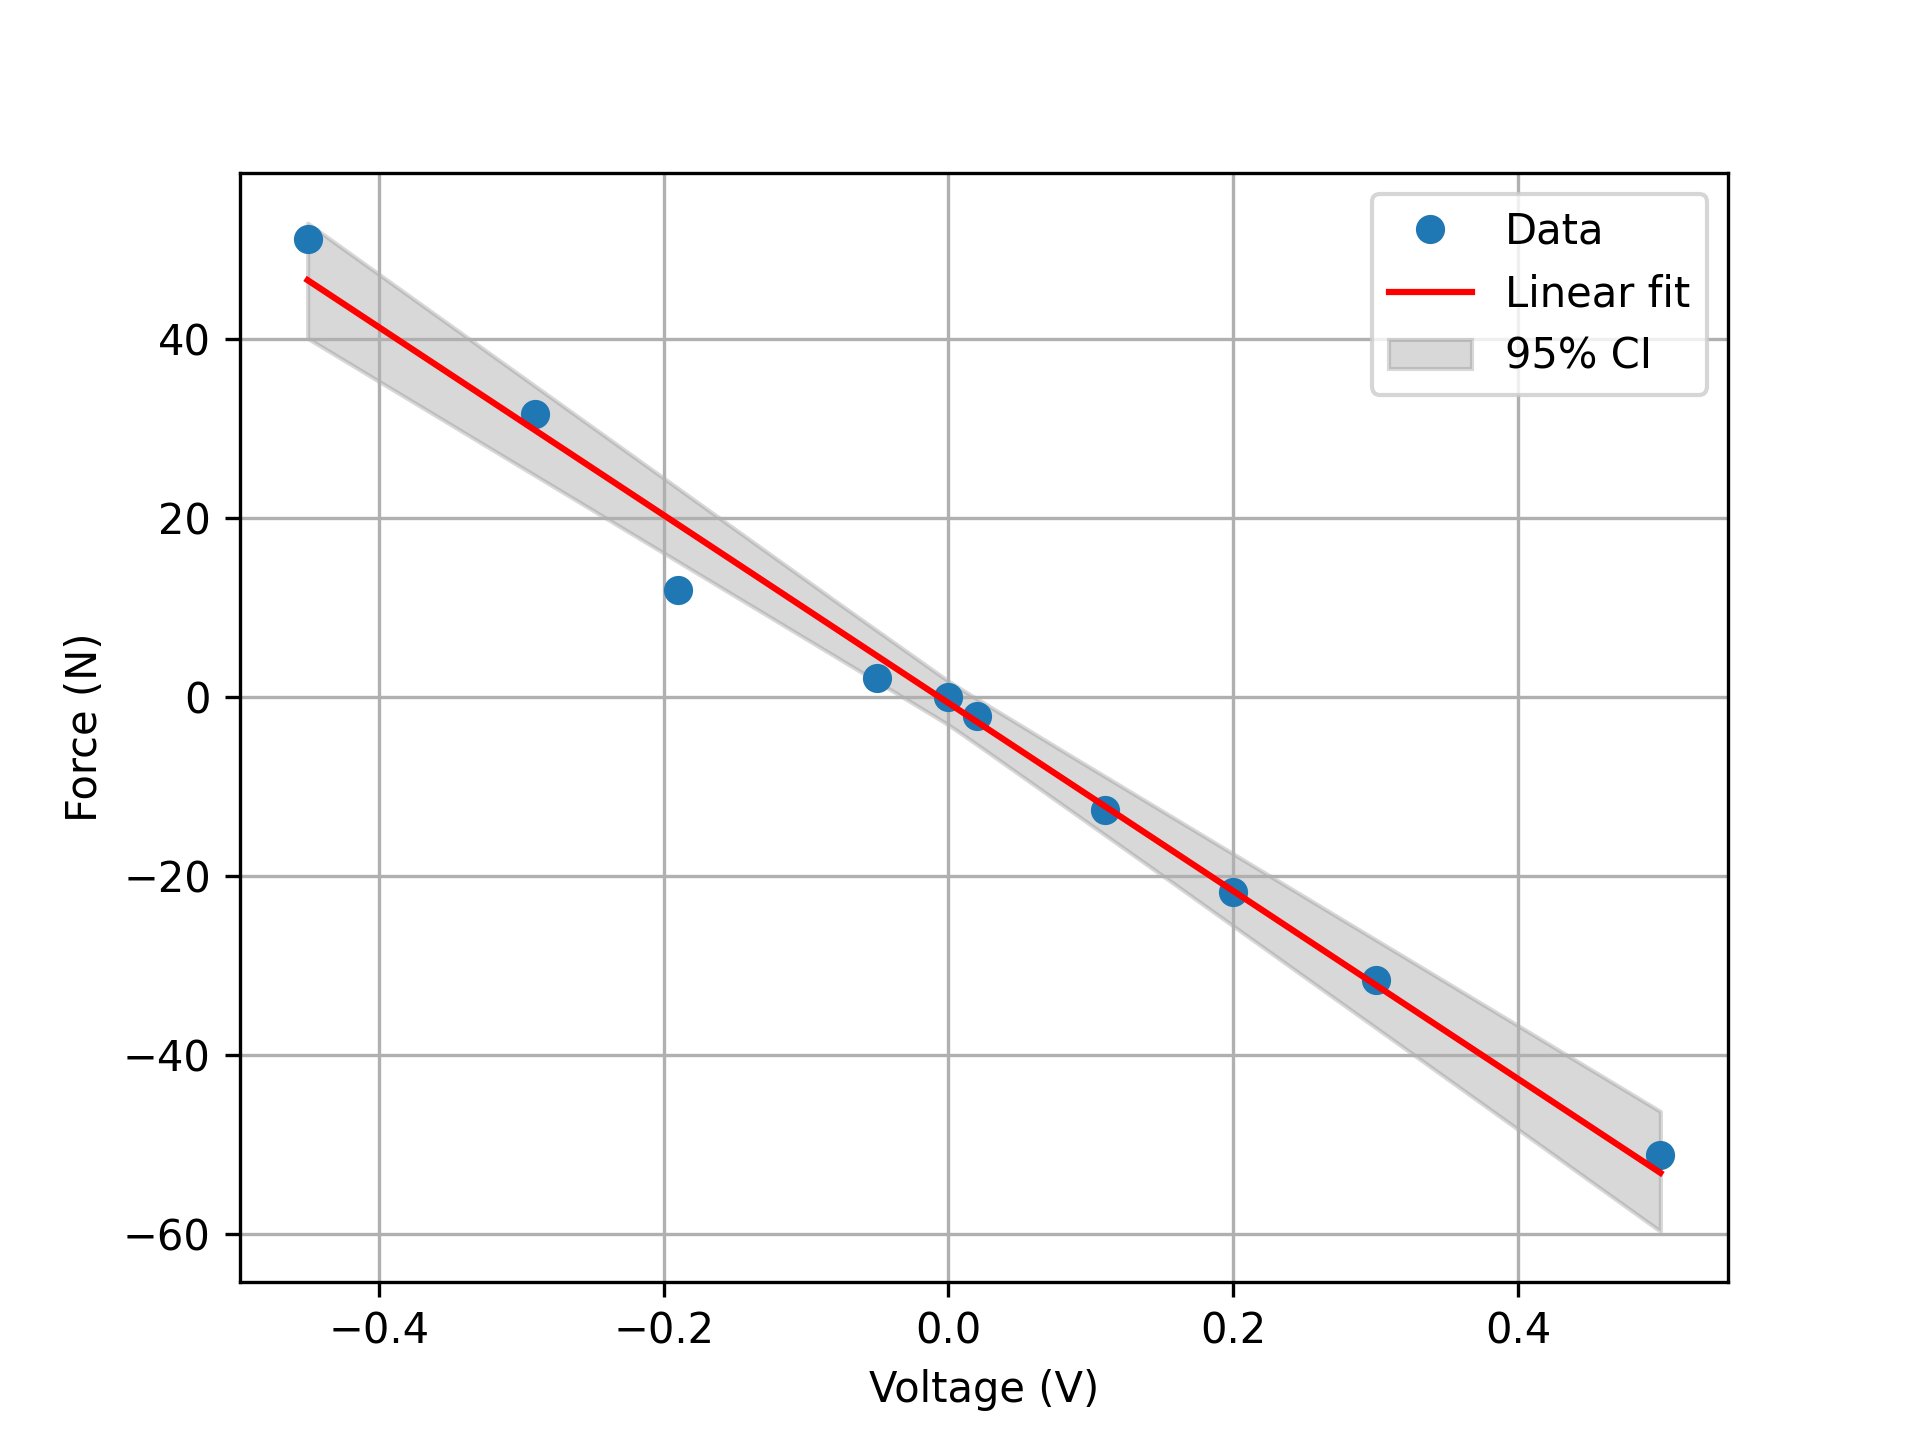
\includegraphics[width=0.8\textwidth]{Calibration/linearity.png}
    \caption{Lateral force transducer voltage calibration.}
    \label{fig:force_linearity}
\end{figure}

\begin{center}
    \textbf{Comment on the accuracy and linearity of the side force transducer}
\end{center}

The side force transducer consists of strain gauages in a Wheatstone bridge.
It is assumed that the location of strain gauges and the bridge configuration is setup to only measure the side force and not be affected by transverse forces.
This was not verified in the experiment as calibation was only done by applying known side forces.

The calibation line in figure \ref{fig:force_linearity} shows a strong linear relationship in the range of forces considered with an $r$ value of -0.9944.
The 95\% confidence interval for the linear fit is shown in the shaded region of the figure.
The uncertainty in forces is negligible and for voltage collected at 2 d.p. $\pm 0.005 V$ is also small.
This indicates both good accuracy and linearity of the transducer.

\subsection{\textbf{Effect Of Speed On Side Force}}

\begin{figure}[H]
    \centering
    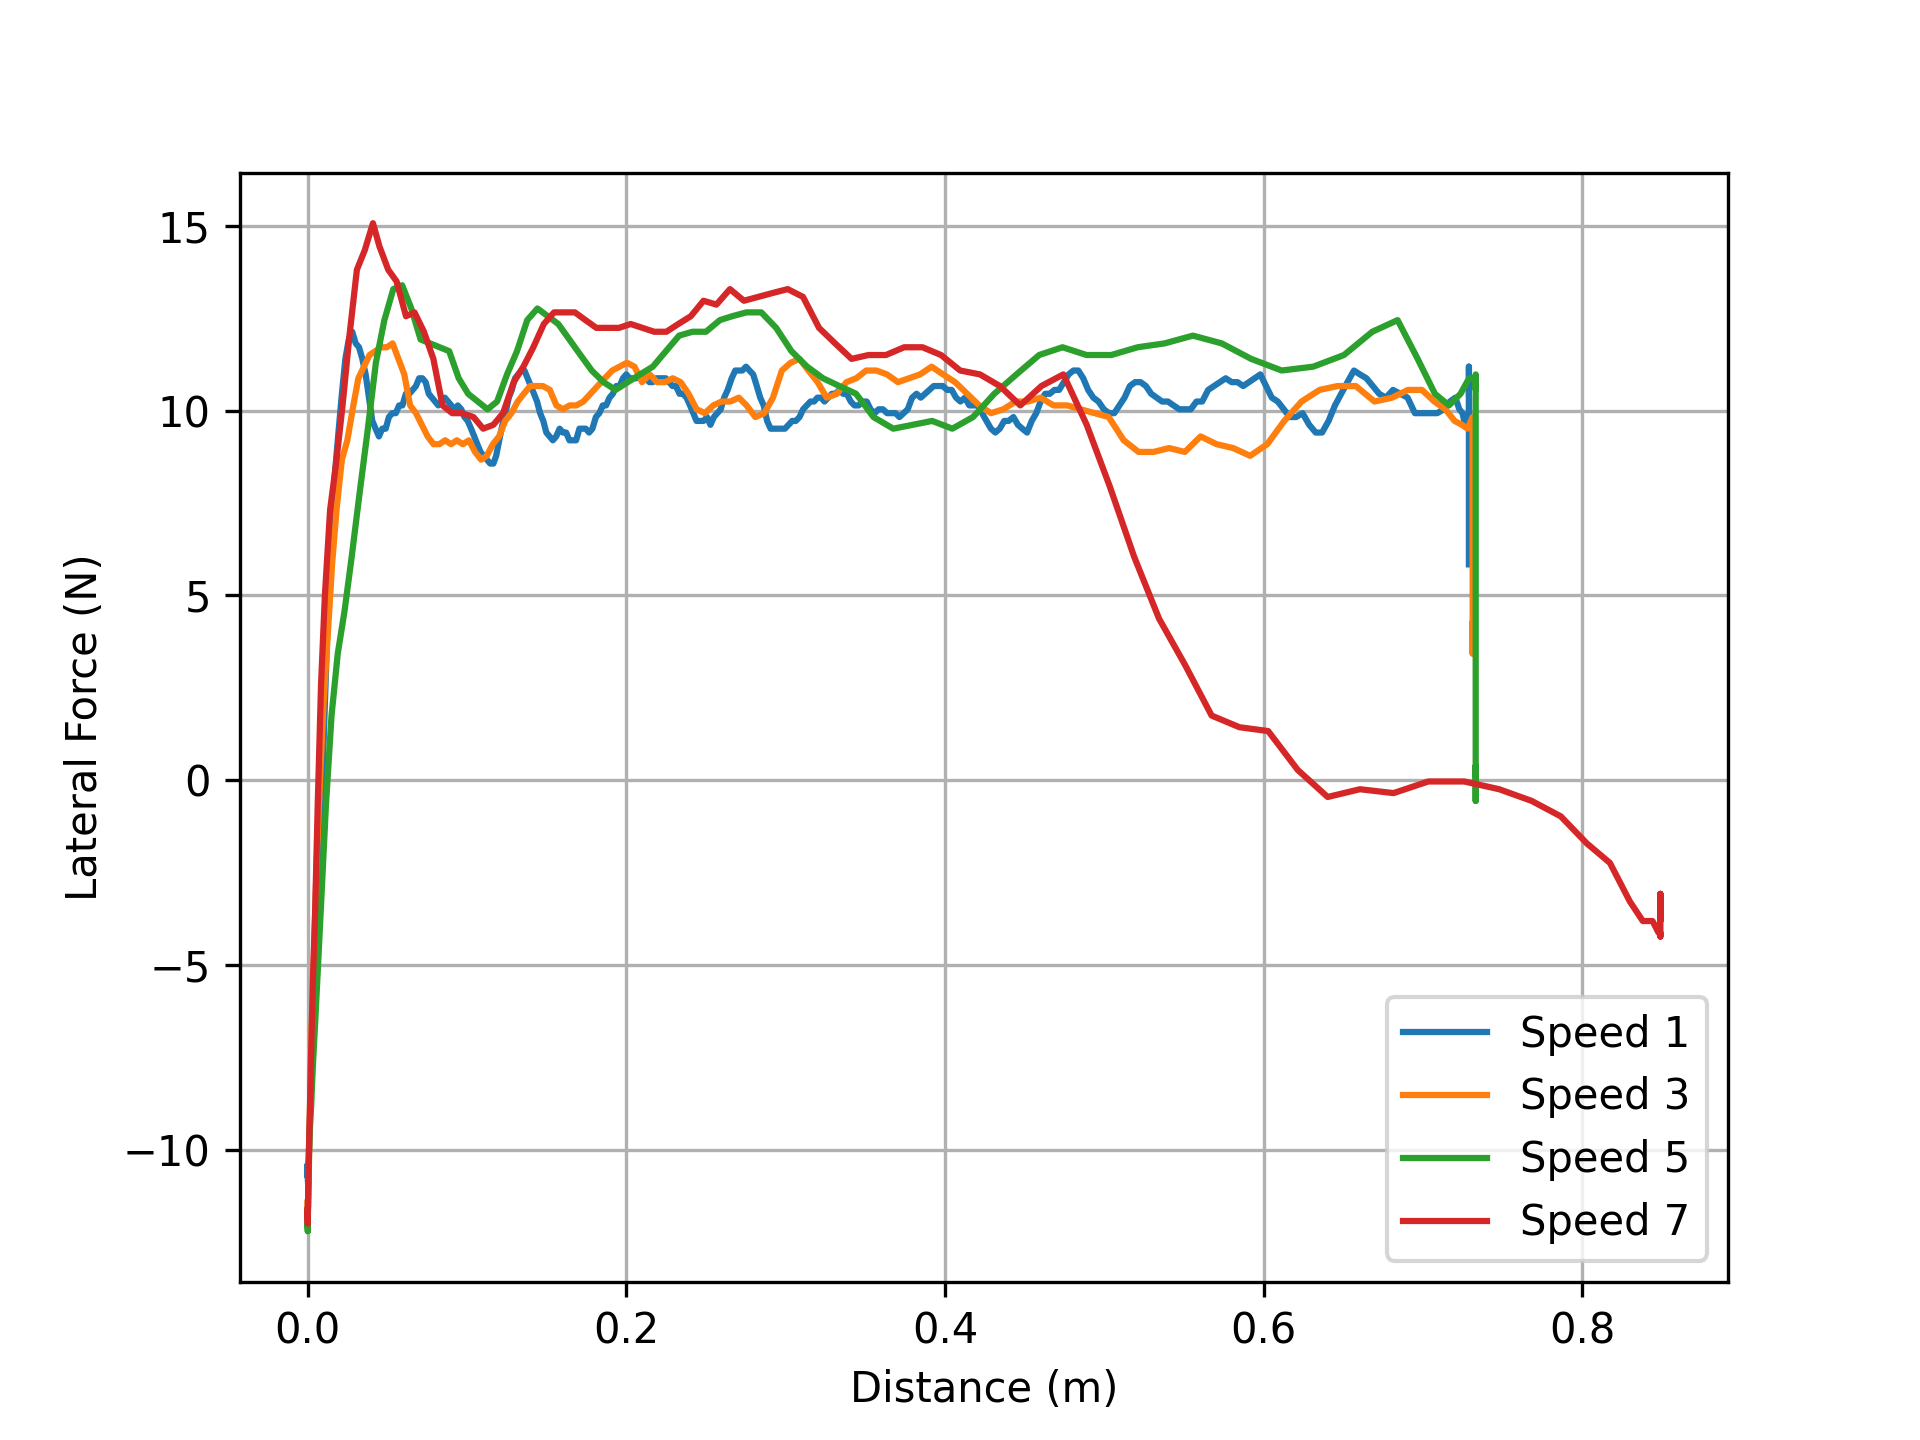
\includegraphics[width=0.8\textwidth]{4.2/force_distances.png}
    \caption{Lateral force vs. distance at $\delta = 5^\circ$ for different rolling speeds.}
    \label{fig:lateral_force_distance_speed}
\end{figure}

\begin{center}
    \textbf{Comment on the influence of rolling speed on the average steady state lateral forces
    developed by the model tyre.}
\end{center}

Figure \ref{fig:lateral_force_distance_speed} shows the sampled lateral force at different rolling speeds as a function of distance.
The motors speed settings \texttt{[1,3,5,7]} at fixed sample rate correspond to a number of samples to cover the full length of track \texttt{[469,134,84,83]}.
The respective average lateral forces are \texttt{[9.31, 10.12, 10.68, 11.73]}.
This shows for a ~250\% increase in speed, the average lateral force increases only 8.7\%.
Speed 7 shows an increased distance to the end of the track which may indicate that the rotary encoder slipped upon the sudden deceleration of the track.
More interestingly at speed 7, a significant drop in lateral force towards the end of the track is observed.
The cause of this is not known.

\subsection{\textbf{Effect of Normal Load on Steady State Side Force}}

\begin{figure}[H]
    \centering
    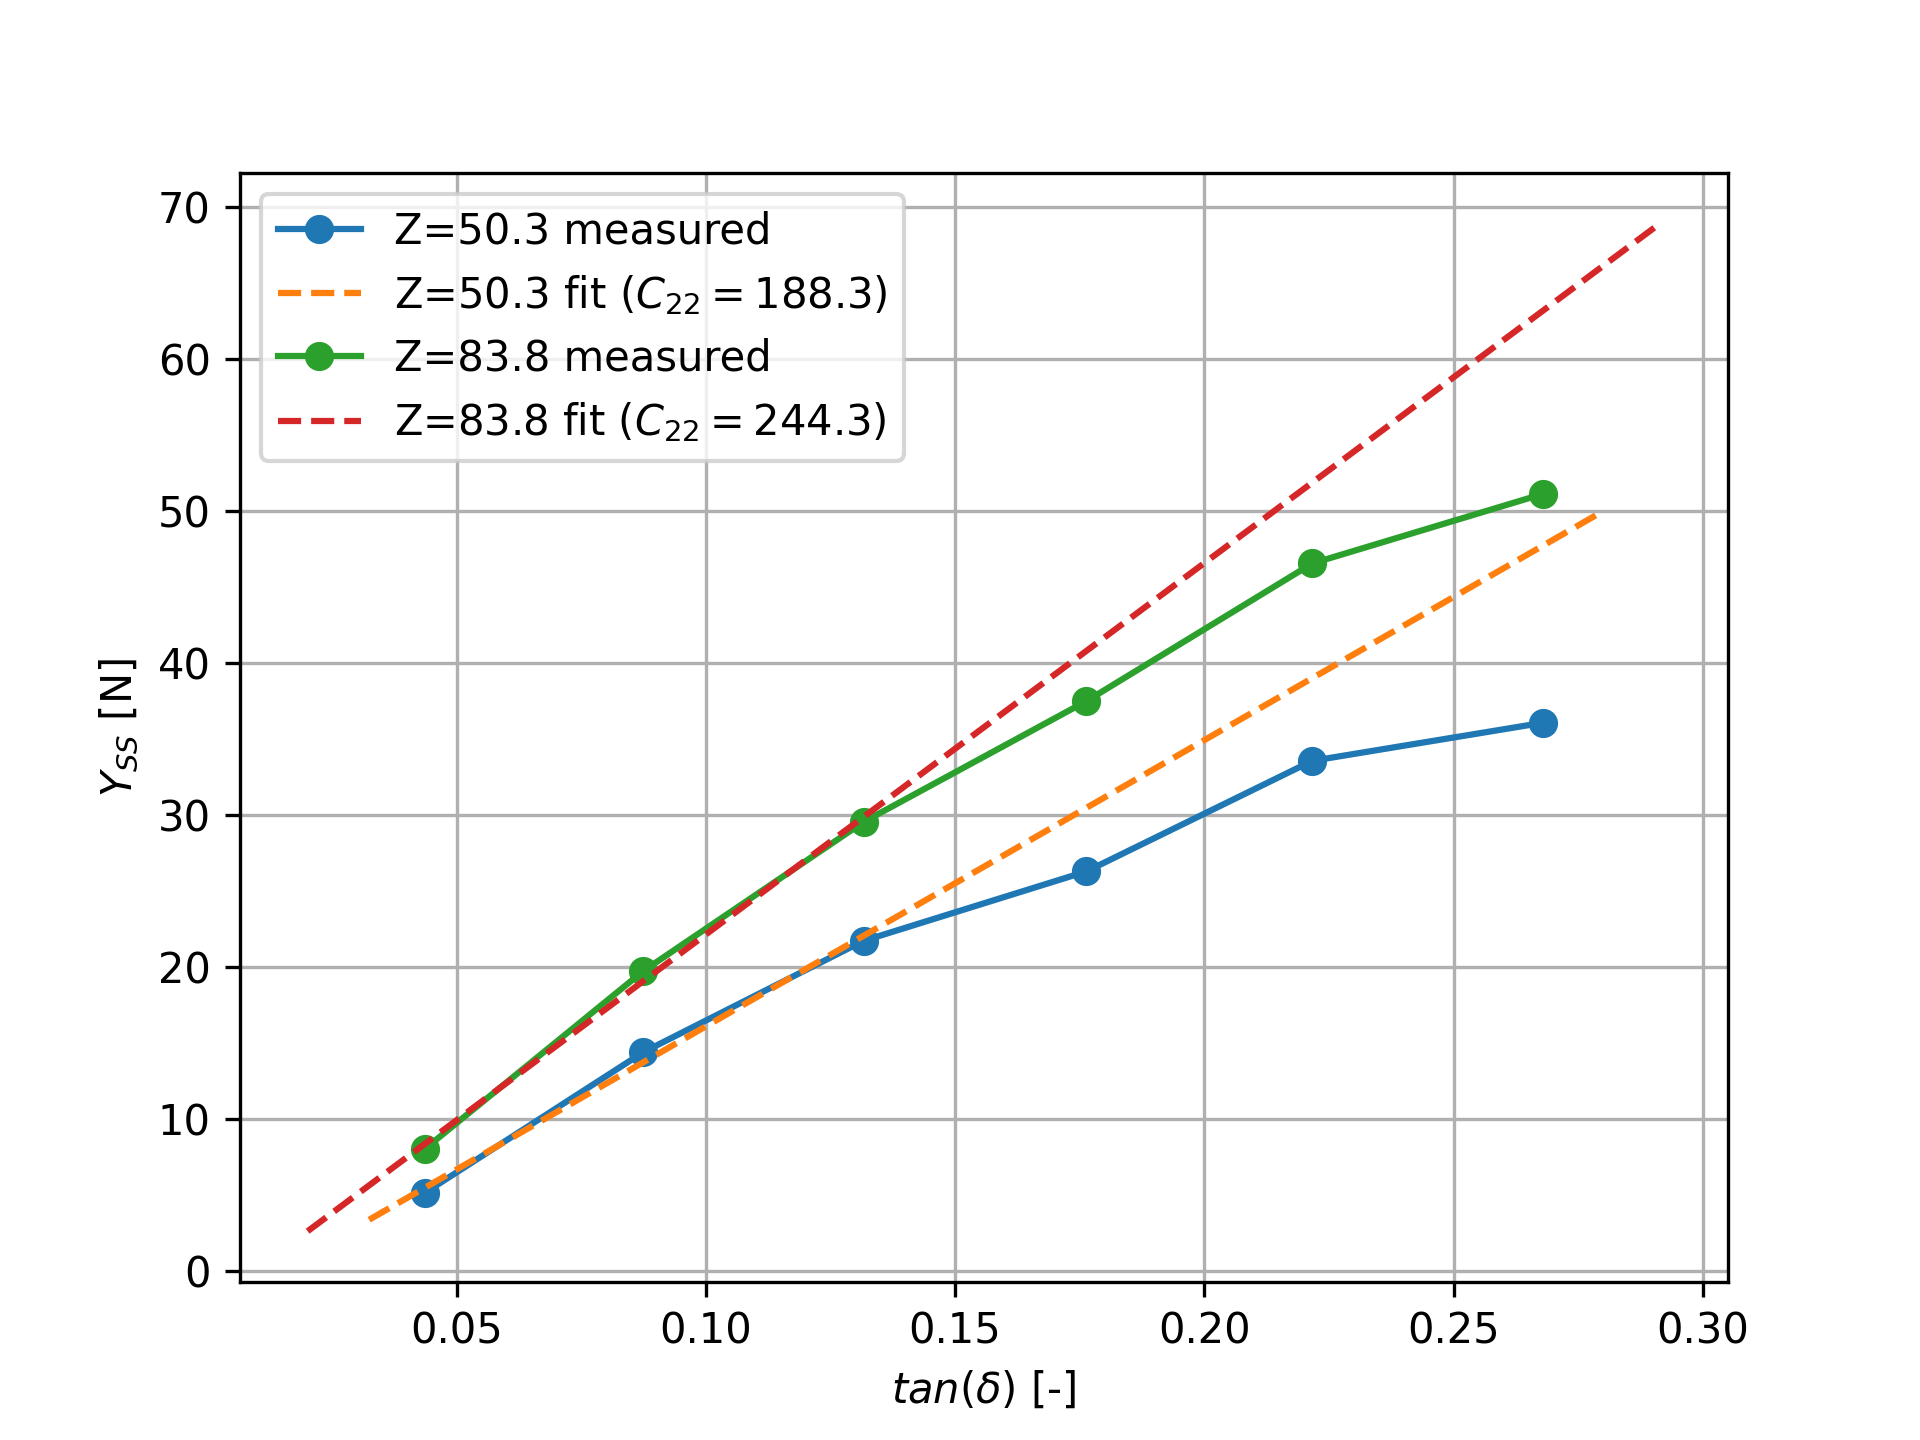
\includegraphics[width=0.8\textwidth]{4.3/Yss_vs_tandelta.png}
    \caption{Lateral force vs. tangent of steer angle.}
    \label{fig:Y_vs_alpha}
\end{figure}

\begin{figure}[H]
    \centering
    \begin{subfigure}{0.3\textwidth}
        \centering
        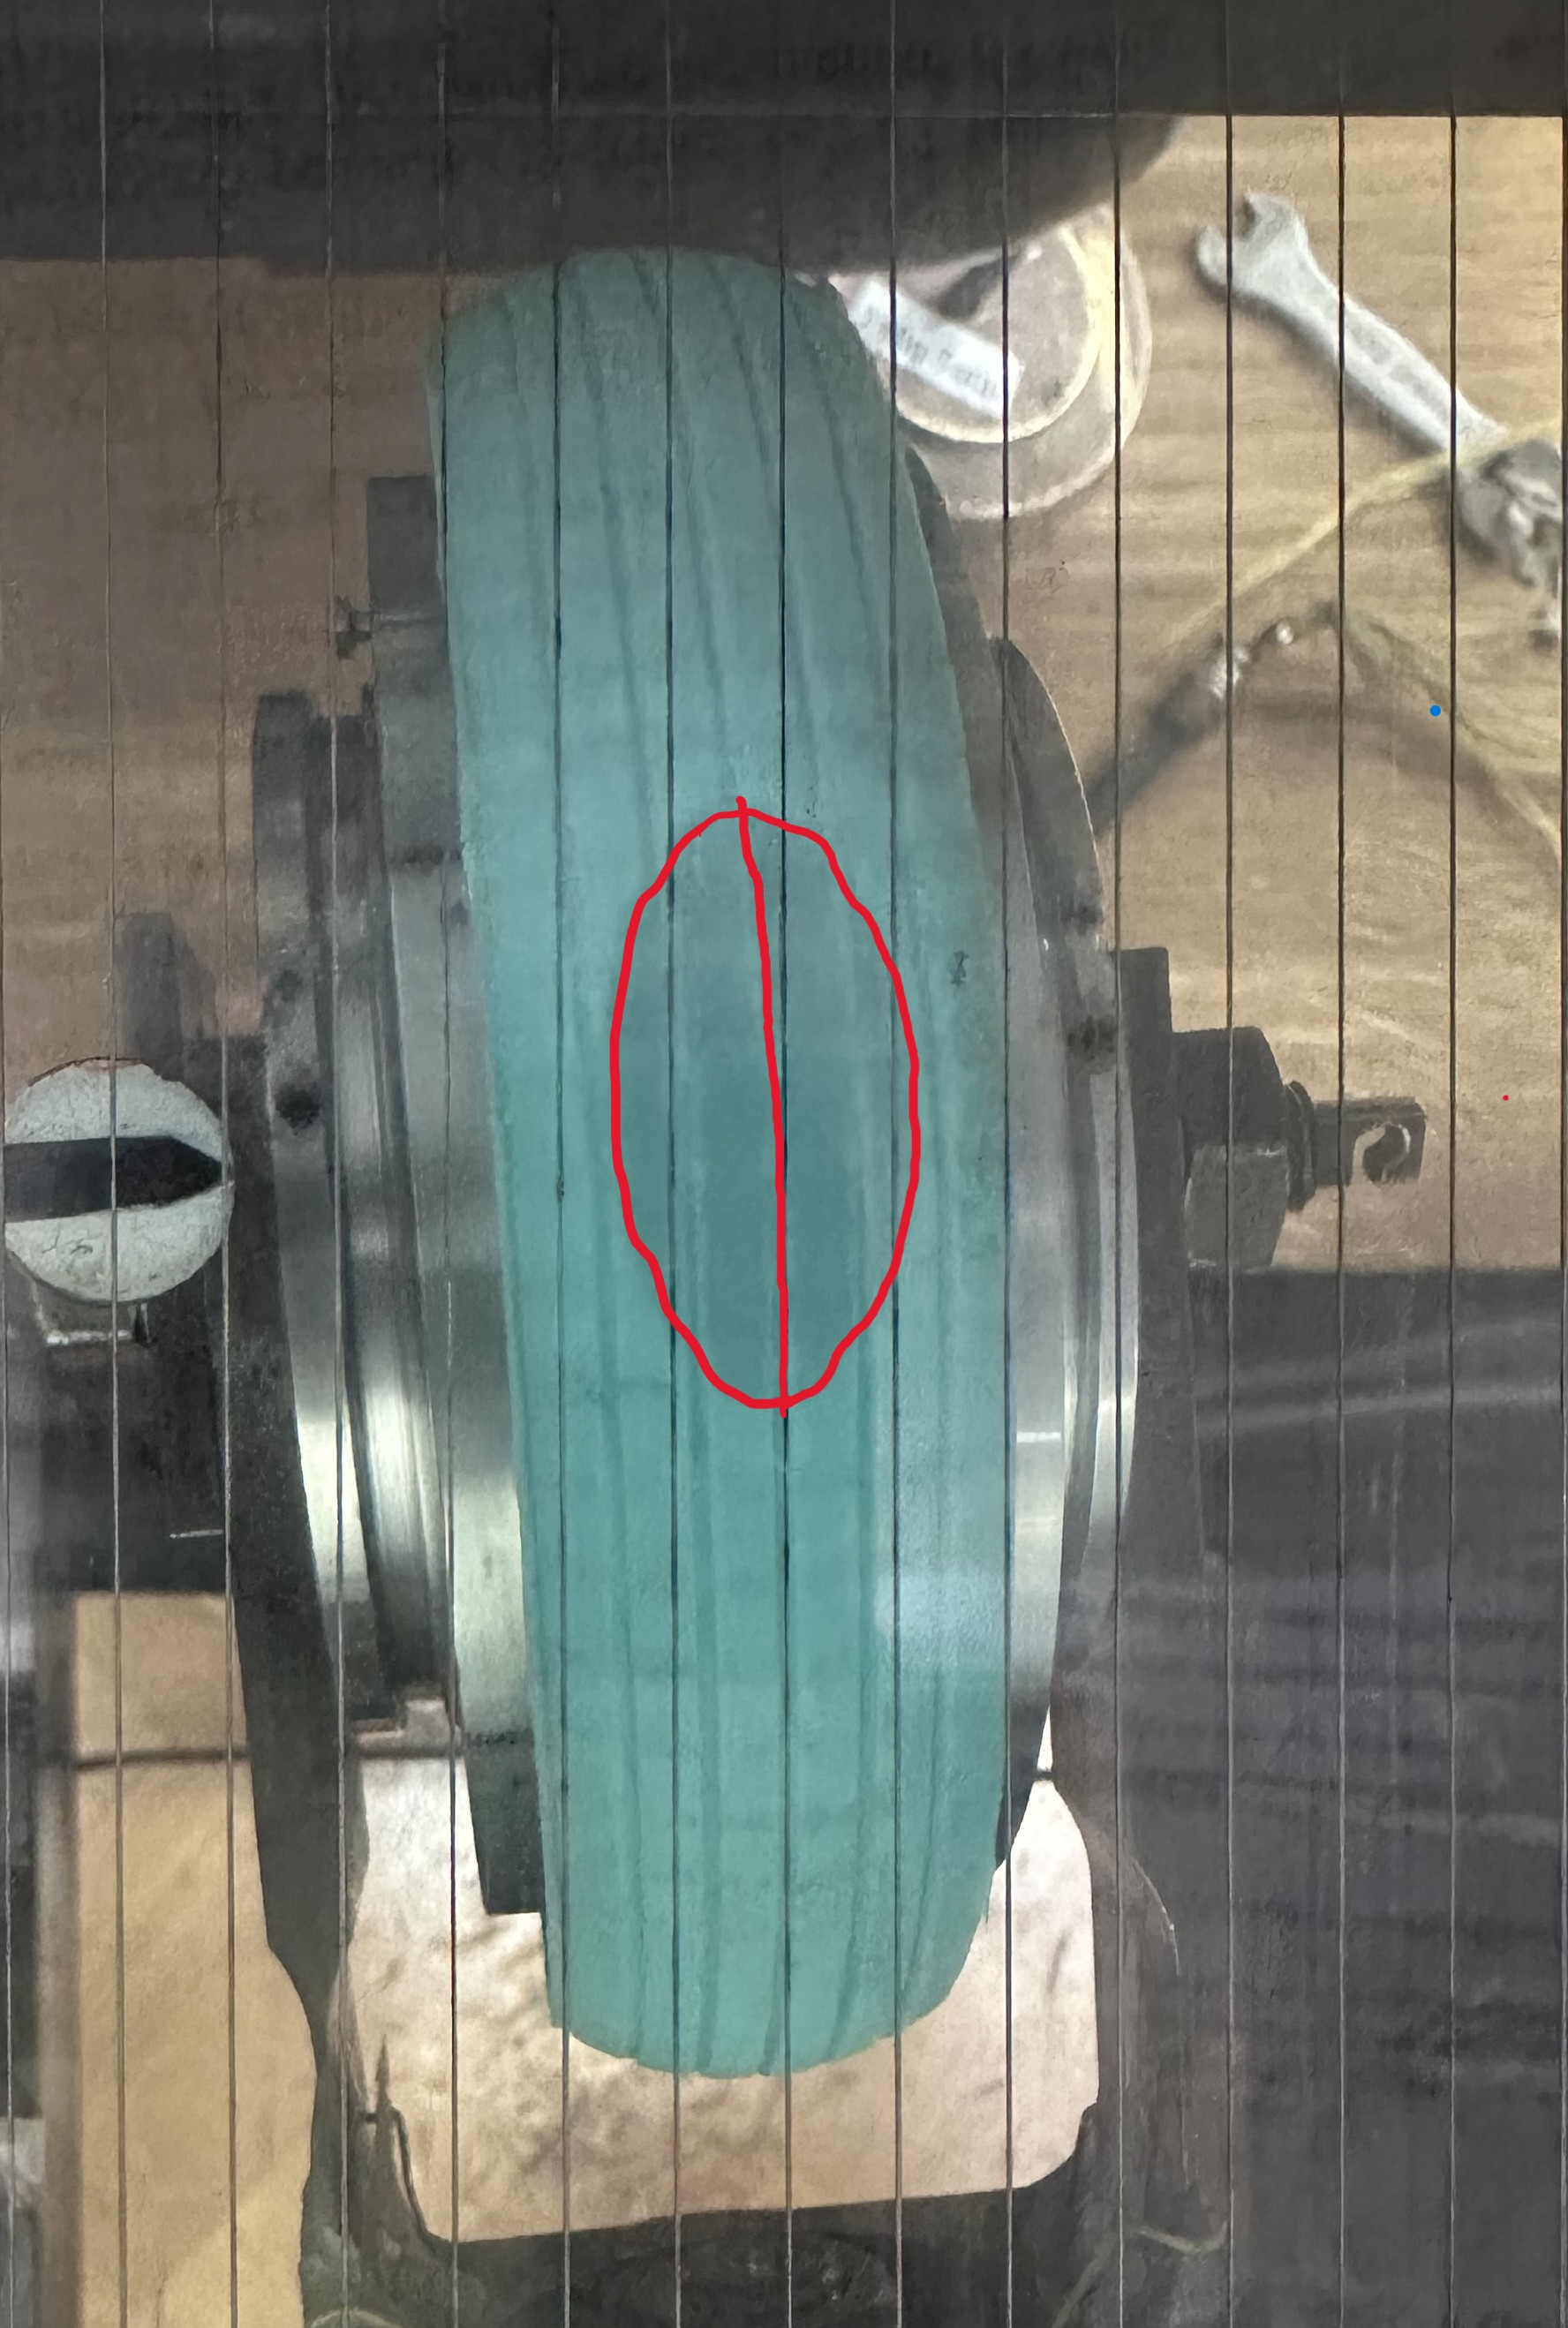
\includegraphics[height=7cm]{photos/5an.jpg}
        \caption{$\delta = 5^\circ$}
        \label{fig:contact_5}
    \end{subfigure}
    \begin{subfigure}{0.3\textwidth}
        \centering
        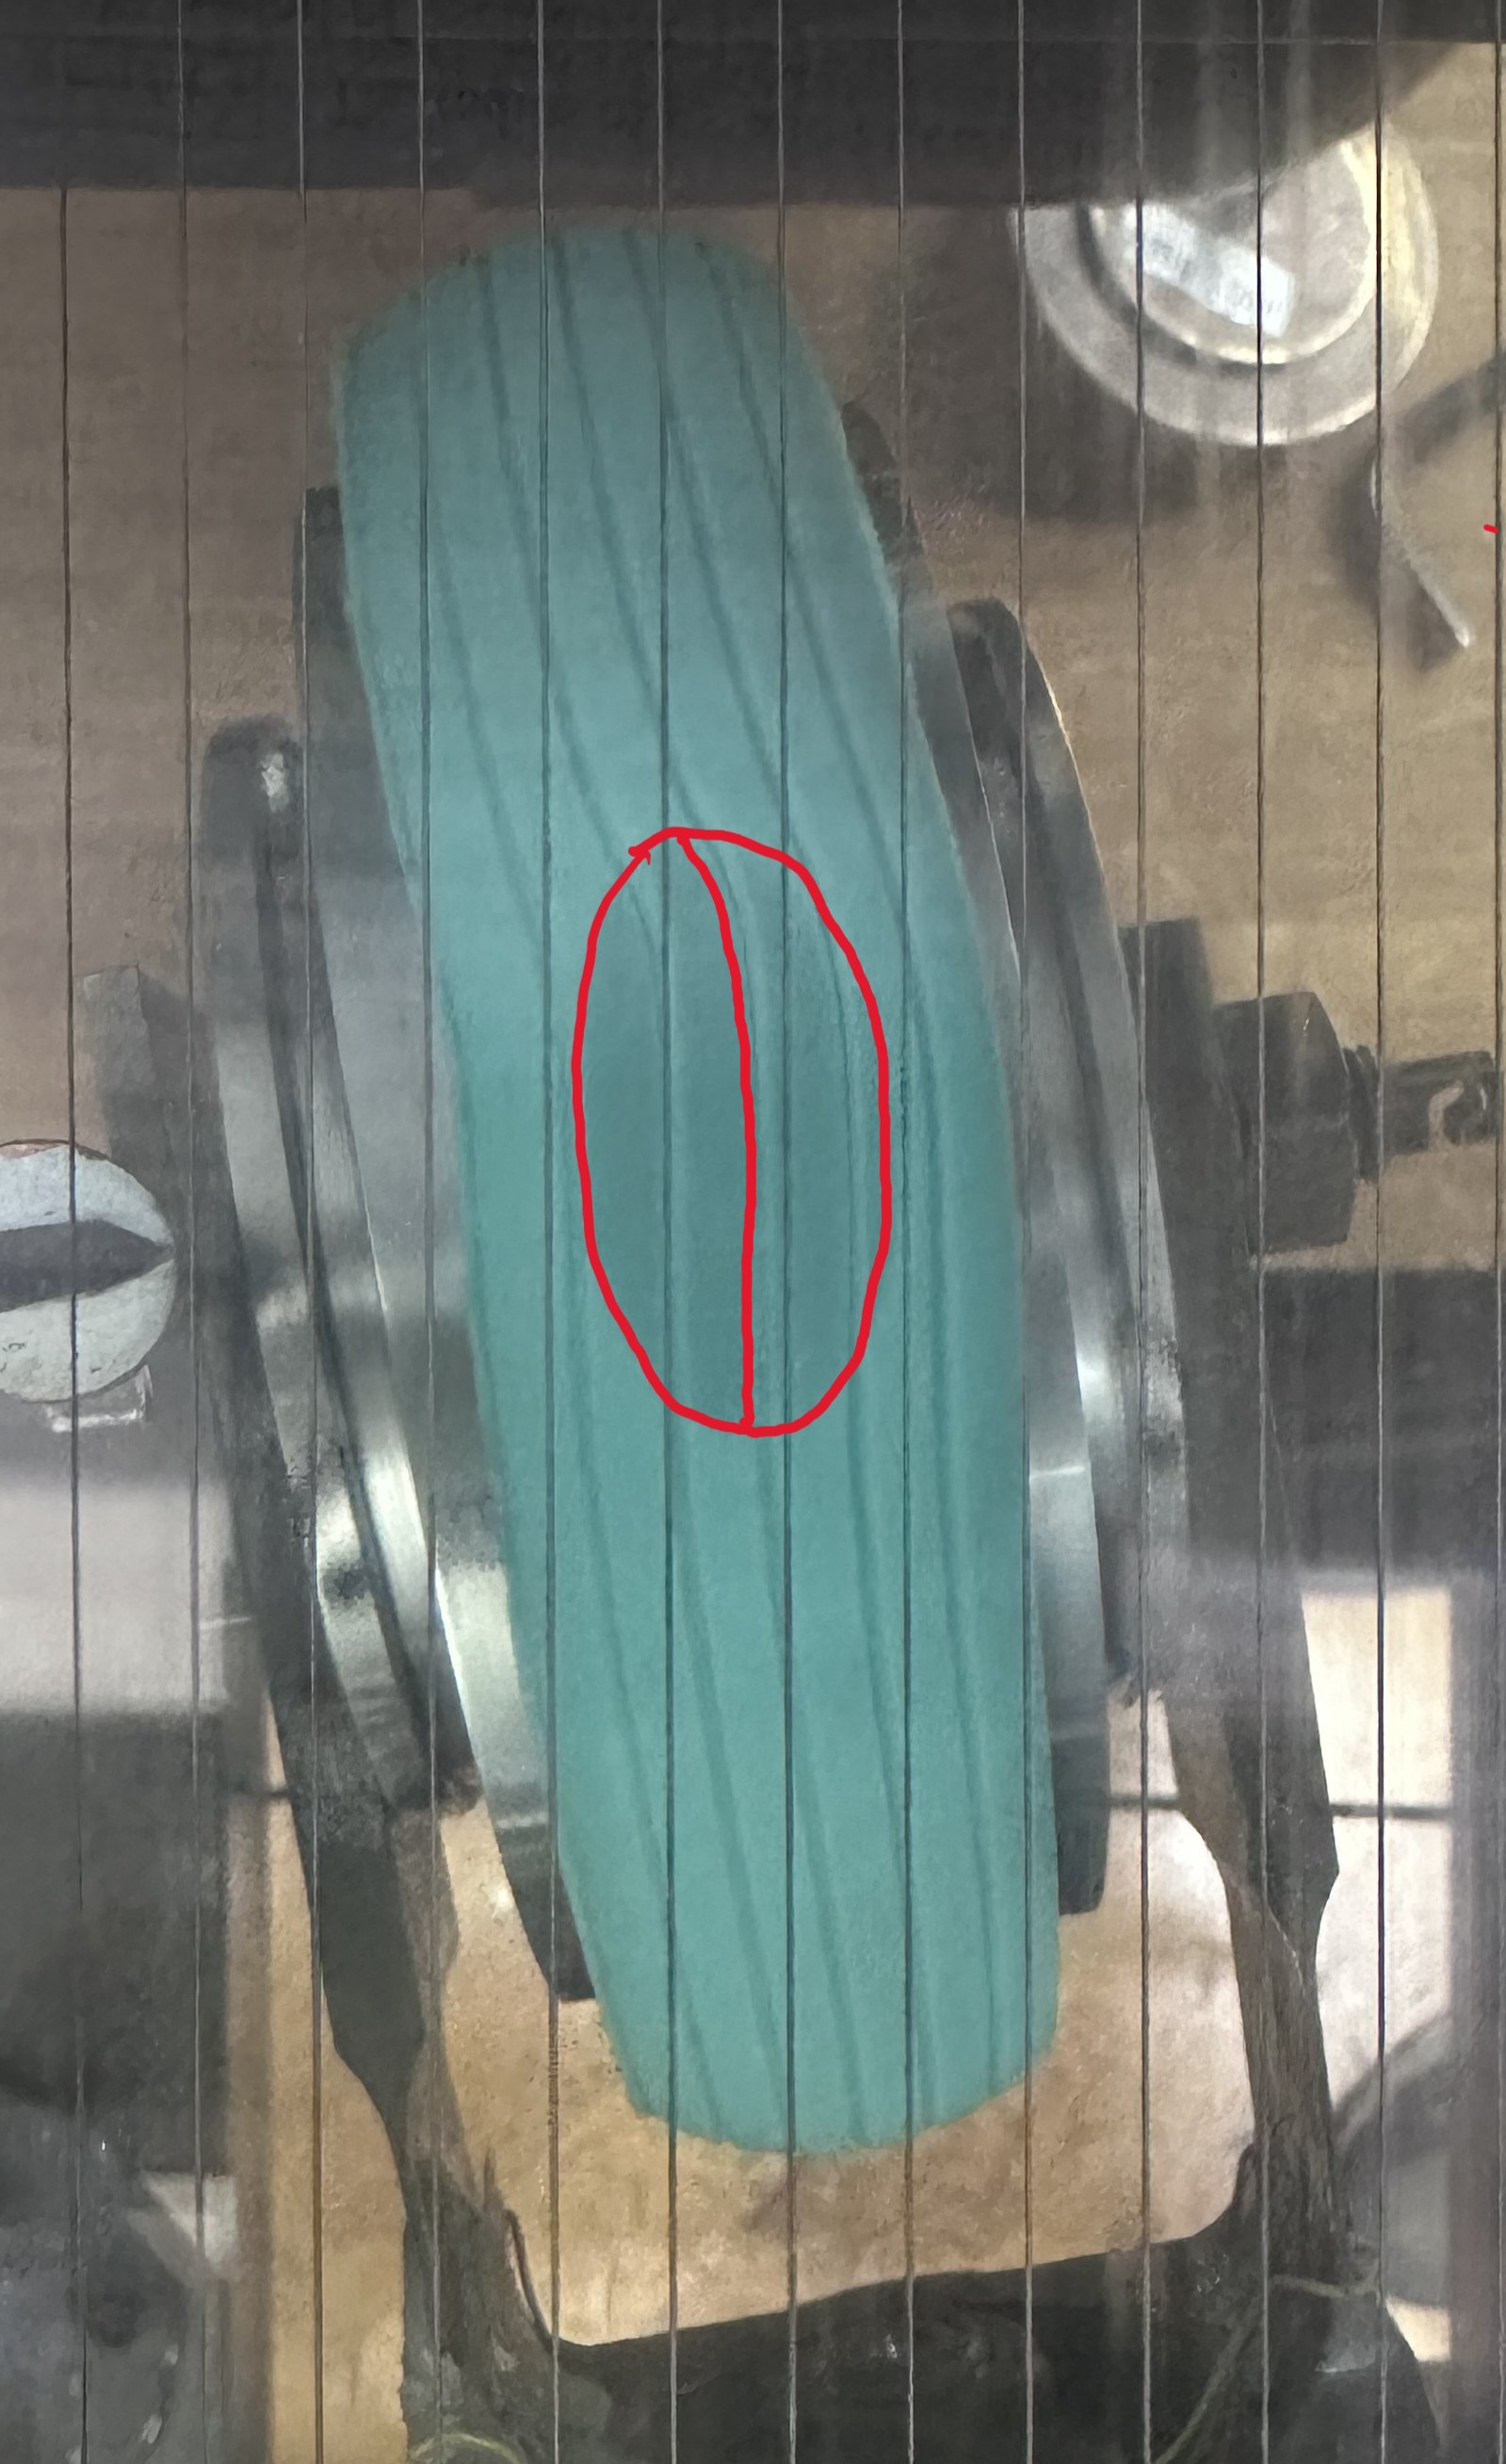
\includegraphics[height=7cm]{photos/10an.jpg}
        \caption{$\delta = 10^\circ$}
        \label{fig:contact_10}
    \end{subfigure}
    \begin{subfigure}{0.3\textwidth}
        \centering
        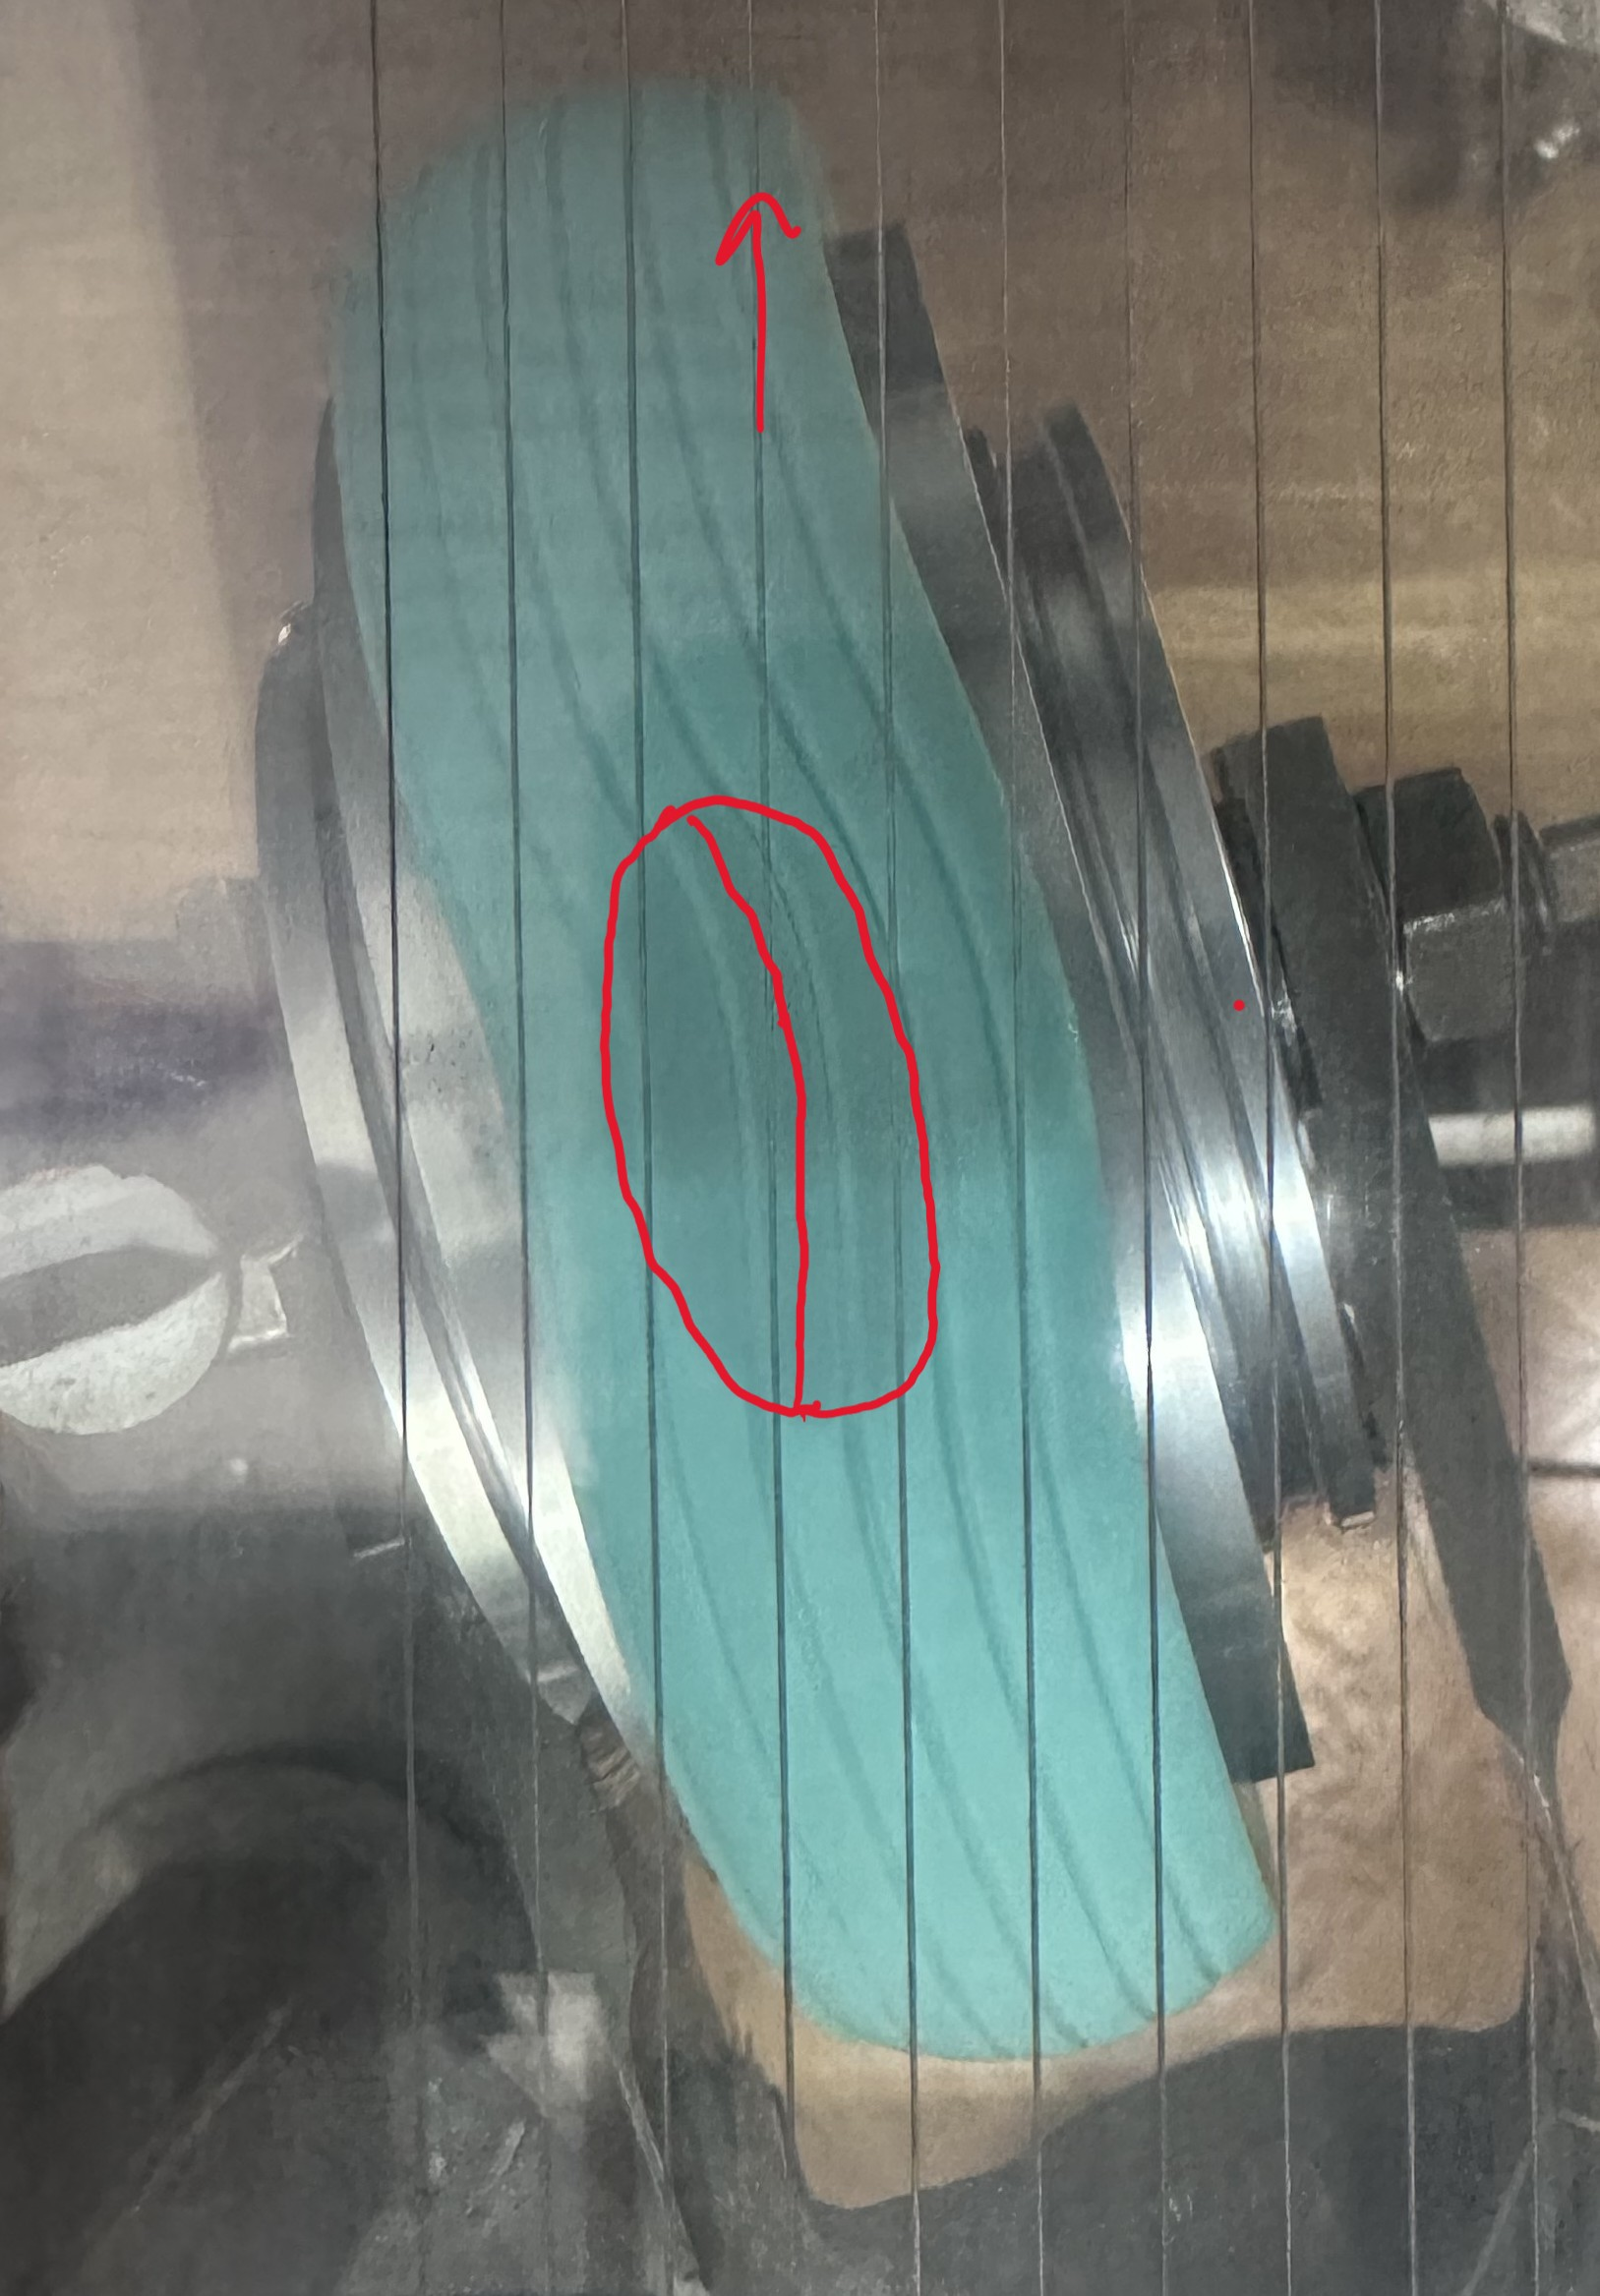
\includegraphics[height=7cm]{photos/15an.jpg}
        \caption{$\delta = 15^\circ$}
        \label{fig:contact_15}
    \end{subfigure}
    \caption{Plan view of wheel contact area for different steer angles.}
    \label{fig:contact_photos}
\end{figure}

\begin{center}
    \textbf{What causes the microslip?}
\end{center}
Microslip occurs where local frictional forces are insufficient to deform the tyre any further and so the tyre slips locally.

\begin{center}
    \textbf{Comment on the relationship between the amount of microslip in the contact area and
    the shape of the Y vs. $ \alpha $ graph}
\end{center}

Figure \ref{fig:Y_vs_alpha} shows a region of linearity between lateral force and steer angle before deviating at high steer angles.
This loss of linearity is due to the onset of microslip.
Figure \ref{fig:contact_photos} shows the contact area of the wheel at different steer angles and the deformed line of the tyre. % TODO: deformed line? centerline? clarify
Figure \ref{fig:contact_5} shows the contact area at a low steer angle which from the bottom, or leading edge, has a line that follows the line on the road surface.
The constant steer angle causes the deformation of the tyre to increase with length from the contact patches leading edge.
Towards the trailing edge the force required to maintain contact exceeds the frictional limit and microslip occurs.
this causes the line of the tyre to deviate from the road surface.
This is seen more clearly in figure \ref{fig:contact_10} and \ref{fig:contact_15} where the deviation from the road surface is more pronounced.
This is due to the increased steer angle requiring more deformation of the tyre to maintain contact, and thus reaches the frictional limit closer to the leading edge of the contact area.
It then follows that the more microslip that occurs, the further the lateral force deviates below the linear regime as a larger area reaches the frictional limit.
% probably worth explaining why it still increases?

The initial gradient $C_{22}$ appears to increase slightly with normal load which is discussed in the next section.

\begin{center}
    \textbf{At which normal load is the tyre nearest to sliding for large
    $ \alpha $ ? Why? How is the
    linear range of Y vs.
    $ \alpha $ affected by the normal load?}
\end{center}

The tyre with a smaller normal load will slide at a smaller steer angle than the higher normal force.
This is because with a smaller normal load the friction limit is reduced and so the peak lateral force occurs at a lower steer angle.
In the brush model, and for microslip occuring strictly in the lateral direction, the peak lateral force would occur when microslip occurs over the entire contact area.
However, in a more realistic model the difference between static and dynamic friction causes the peak lateral force to occur microslip occurs over only a portion of the contact area.

The gradient of the initial linear range should not be affected by the normal load as the tyre should be in the linear elastic regime.
However, the reduced gradient of the smaller normal load tyre does indicate that more microslip is present and so its closer to sliding.

\section{LONGITUDINAL CREEP}

\subsection{\textbf{No Load Creep} \label{no_load_creep}}

A no load creep test is performed at each normal load to determine the effective rolling radius of the tyre.
This will change with normal load as the tyre deforms more under higher loads.
For Z = 50.3 N, the effective radius is 45.1 mm and for Z = 83.8 N, the effective radius is 44.7 mm.

\subsection{\textbf{Creep with an Applied Torque}}

\begin{figure}[H]
    \centering
    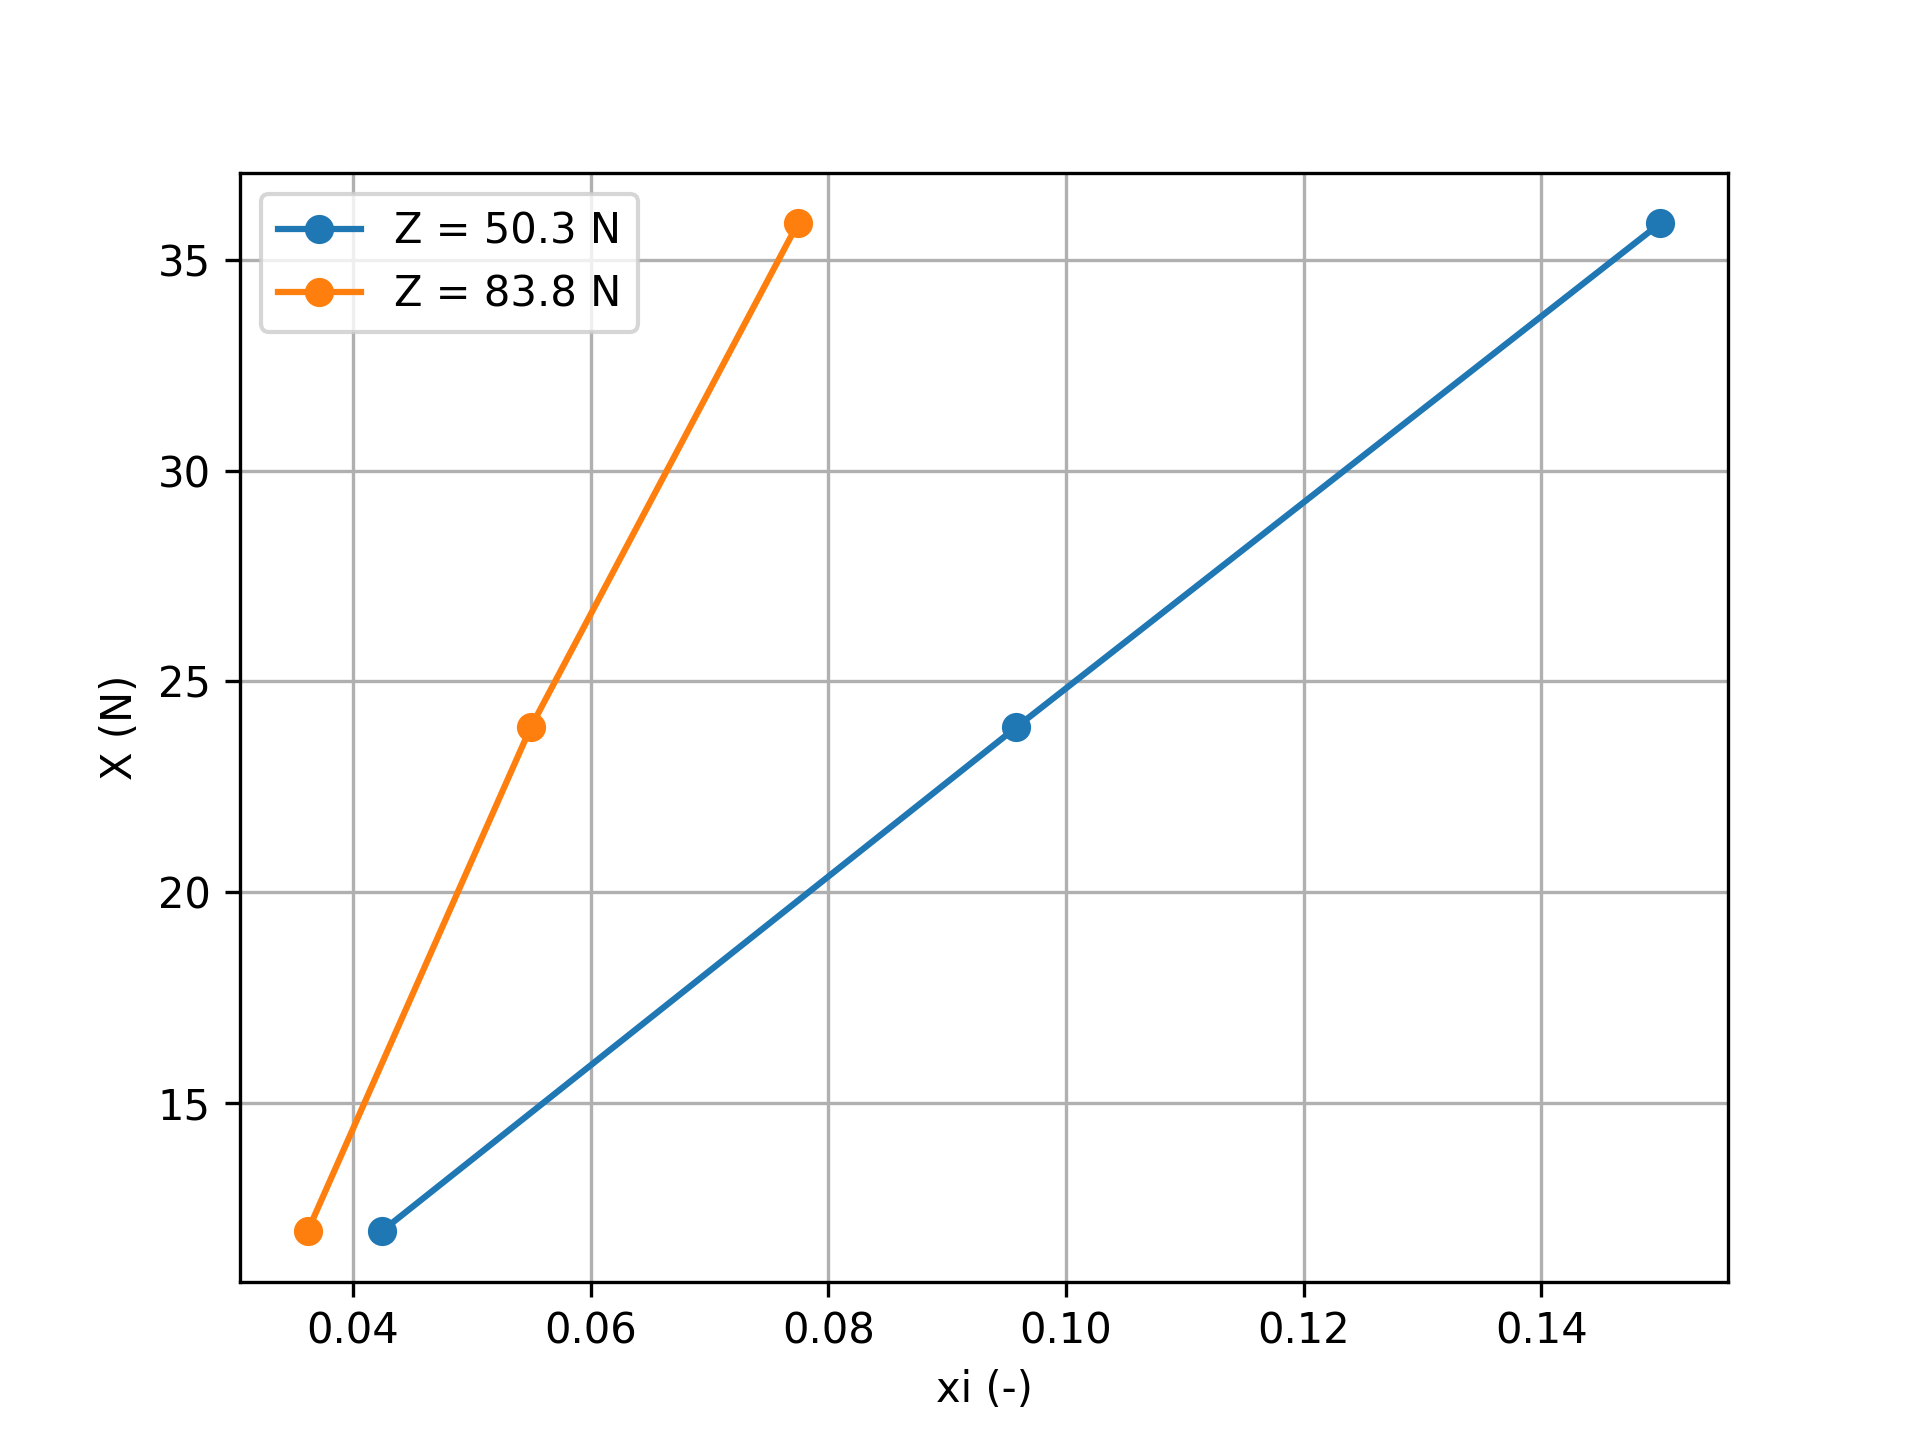
\includegraphics[width=0.8\textwidth]{52.png}
    \caption{Longitudinal force vs longitudinal creepage for different loads.}
    \label{fig:longitudinal_force_vs_creepage}
\end{figure}

\begin{center}
    \textbf{ Comment on the longitudinal deformation and compare it with the lateral deformation
    in section 4.3. Where is sliding most likely to occur? Comment also on the
    relationship between the amount of sliding in the contact area and the shape of the X
    vs. ξ graph.}
\end{center}

The longitudinal deformation shown in figure \ref{fig:longitudinal_force_vs_creepage} shows strong linearity at both normal forces measured.
Its important to note that higher creep values were not possible to be measured due to the mass applying the torque reaching the floor during the slip.
The different normal forces have very different gradients with $C_{11}|_{Z=50.3} = 149.7$ N and $C_{11}|_{Z=83.8} = 389.2$ N.
This shows that longitudinal creep coefficient $C_{11}$ increases with the normal force $Z$.

Comparing this to the lateral deformation, 

\subsection{\textbf{Combined Lateral and Longitudinal Creep}}

\begin{figure}[H]
    \centering
    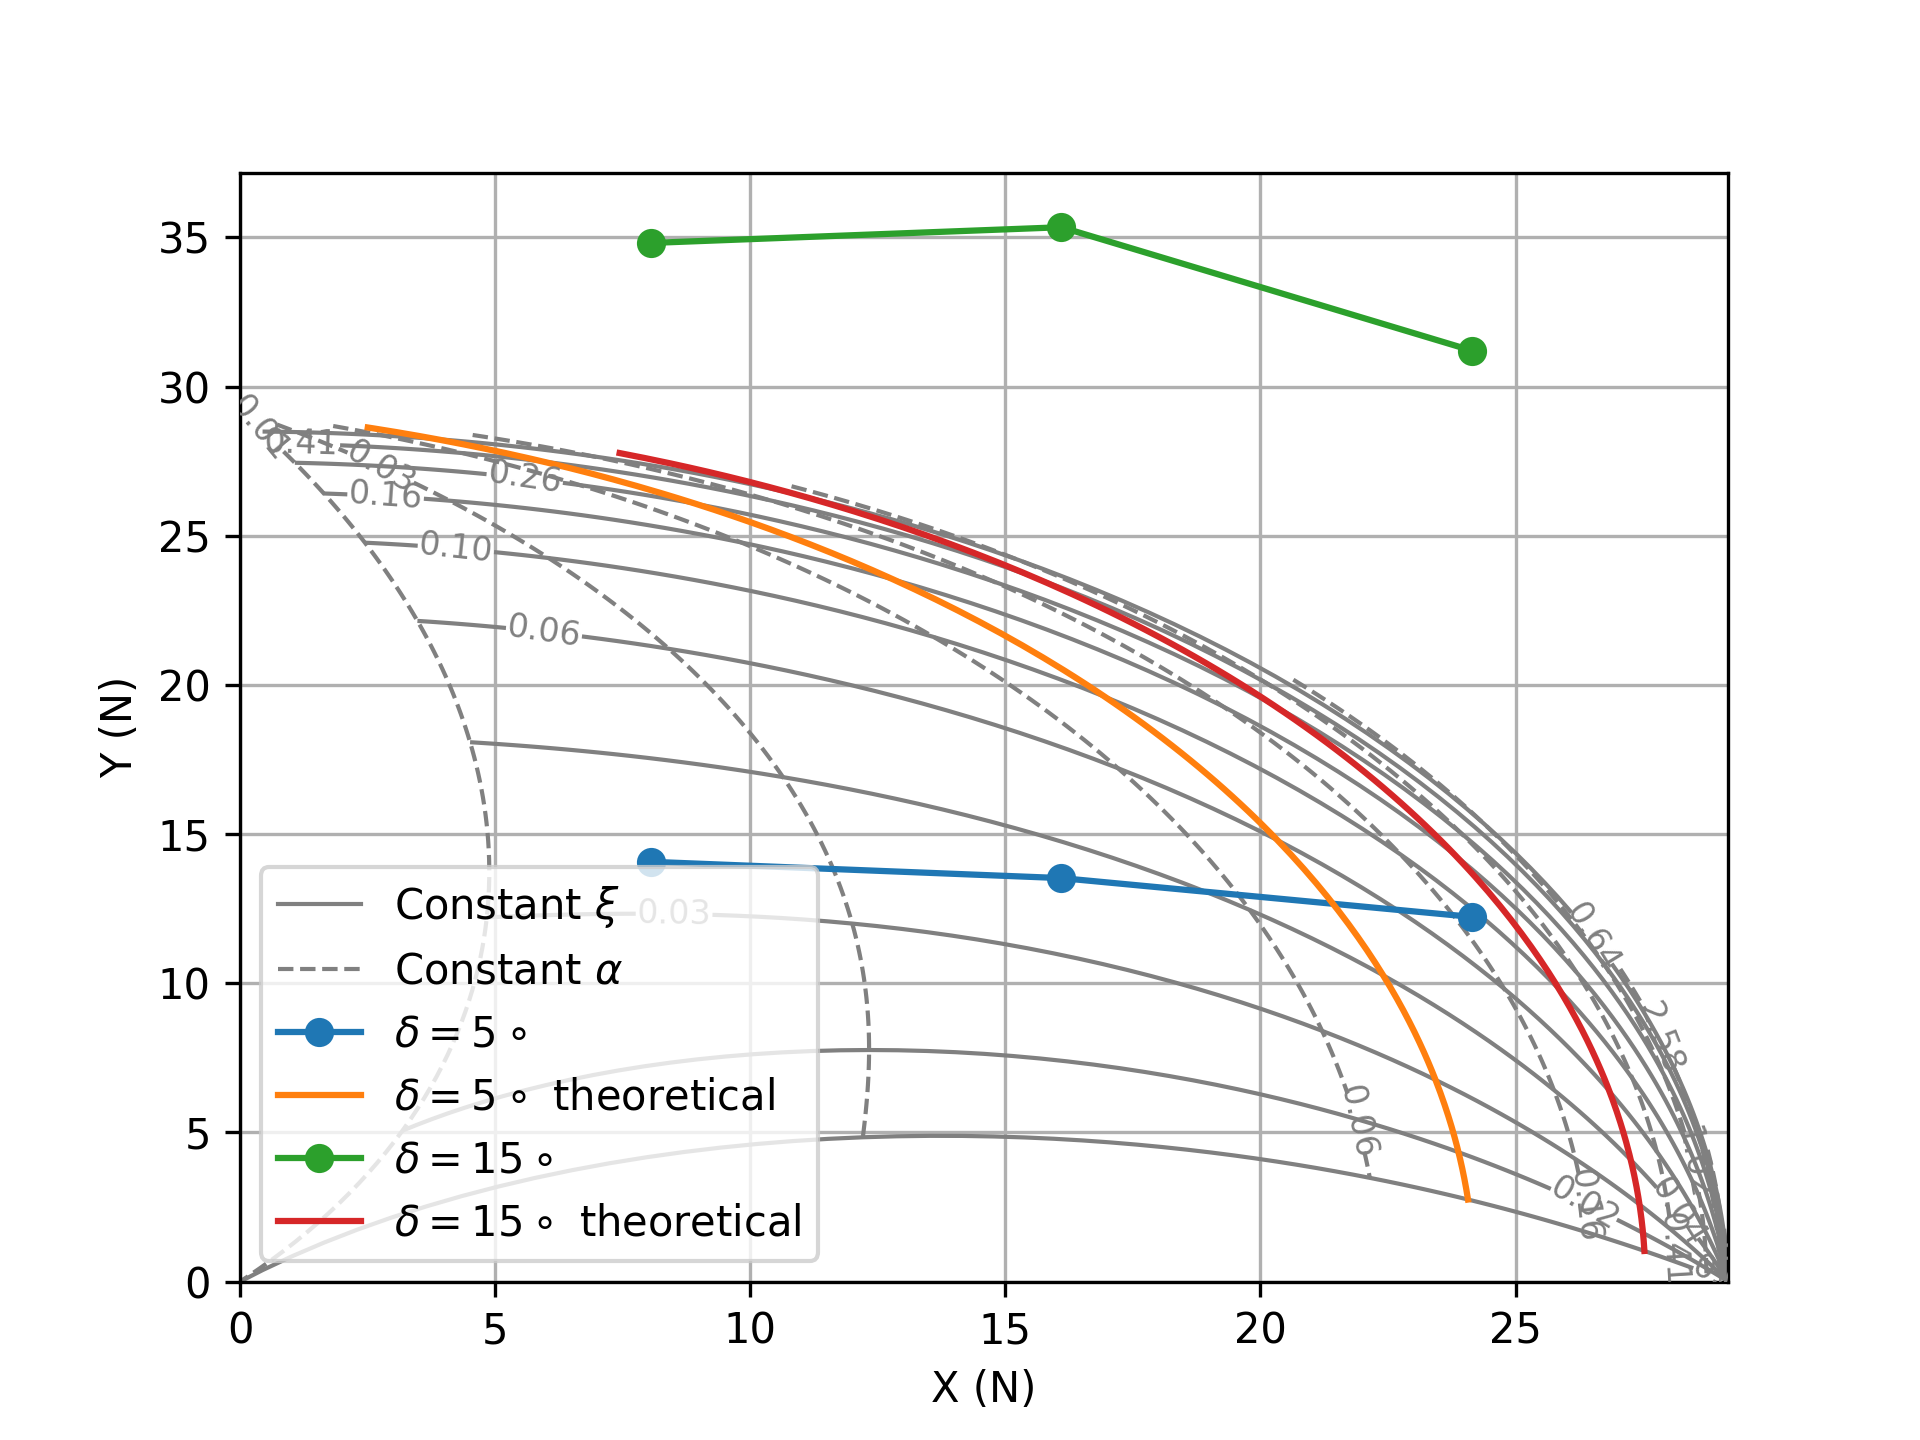
\includegraphics[width=0.8\textwidth]{5.3/XvsY.png}
    \caption{}
    \label{fig:lateral_force_vs_longitudinal_force}
\end{figure}

\begin{center}
    \textbf{Comment on the comparison between theory and experiment.}
\end{center}

\section{Appendix}

The longitudinal creepage is calculated using the equation below
\begin{equation}
    \xi = \frac{\Delta x}{x} 
     = \frac{x_{2} - x_{1}}
            {\bigl(x_{\max} - x_{1}\bigr) + \bigl(x_{\max} - x_{2}\bigr)}.
\end{equation}

The nonlinear model longitudinal and lateral forces are given using the equations below \cite{handout}.
\begin{align}
Y &= \mu Z \,\frac{\alpha}{\sqrt{\xi^2 + \alpha^2}}
\left[\,1 - \frac{\xi_0}{2\,\sqrt{\xi^2 + \alpha^2}}\,\right] \\
    X &= \mu Z \,\frac{\xi}{\sqrt{\xi^2 + \alpha^2}}
    \left[\,1 - \frac{\xi_0}{2\,\sqrt{\xi^2 + \alpha^2}}\,\right]
\end{align}

\begin{thebibliography}{9}


  \bibitem{handout}
  X. Na
  \emph{LABORATORY EXPERIMENT: MODEL TYRE TESTS}
  University of Cambridge,
  Feburary 2025.

\end{thebibliography}

\end{document}